\documentclass{article}
\usepackage{graphicx}
\usepackage[style=ieee]{biblatex} % Establecer el estilo de las referencias como IEEE
\usepackage{xcolor}
\usepackage{hyperref}
\usepackage{titletoc}
\usepackage{adjustbox}
\usepackage{amsmath}
\usepackage[spanish]{babel}

\usepackage{listings}
\hypersetup{
    colorlinks=true,
    linkcolor=blue, % Color del texto del enlace
    urlcolor=blue % Color del enlace
}

\usepackage{longtable} % Agrega el paquete longtable

\definecolor{mygreen}{RGB}{0,128,0}

\usepackage{array} % Para personalizar la tabla
\usepackage{booktabs} % Para líneas horizontales de mejor calidad
\usepackage{graphicx} % Paquete para incluir imágenes
\usepackage{float}

% Definir márgenes
\usepackage[margin=1in]{geometry}

\renewcommand{\contentsname}{\textcolor{mygreen}{Tabla de Contenidos}}

\begin{document}

\begin{titlepage}
    \centering
    % Logo de la Universidad
    
\includegraphics[width=0.48\textwidth]{logo_universidad.png}
    \par\vspace{2cm}

    % Nombre de la Universidad y detalles del curso
    {\Large \textbf{Universidad Nacional de Colombia} \par}
    \vspace{0.5cm}
    {\large Ingeniería de Sistemas y Computación \par}
    {\large 2025969 Modelos estocásticos y simulación en computación y comunicaciones (01)\par}
    \vspace{3cm}

    % Detalles del laboratorio y actividad
    {\large \textbf{Taller 1} \par}
    \vspace{3cm}

    % Lista de integrantes
    {\large \textbf{Integrantes:} \par}
    \vspace{0.5cm}
    \begin{tabular}{ll}
    Javier Andrés Tarazona Jiménez & jtarazonaj@unal.edu.co \\
    Yenifer Yulieth Mora Segura & ymoras@unal.edu.co \\
    Juan Esteban Carranza Salazar & jcarranza@unal.edu.co \\
    Grevy Joner Rincon Mejia & grrinconm@unal.edu.co \\
    Jefferson Duvan Ramirez Castañeda & jeramirezca@unal.edu.co \\
    Javier Andres Carrillo Carrasco & jacarrillo@unal.edu.co \\
    Diego Nicolas Ramirez Maldonado & dieramirezma@unal.edu.co \\
    \end{tabular}
    \par\vspace{3cm}

    % Fecha
    {\large Julio 13 de 2025 \par}
\end{titlepage}

\tableofcontents % Inserta la tabla de contenidos

\newpage % Salto de página para separar la tabla de contenidos del contenido del documento

% Contenido del artículo----------------------------------------------------------

%---------------------------------------------------------------------------------
% Intro --------------------------------------------------------------------------
%---------------------------------------------------------------------------------

\section{Introducción}\label{sec:intr}


%---------------------------------------------------------------------------------
% Marco Teórico ------------------------------------------------------------------
%---------------------------------------------------------------------------------

\section{Marco Teórico}\label{sec:marc}


%---------------------------------------------------------------------------------
% Descr. Problema ------------------------------------------------------------------
%---------------------------------------------------------------------------------

\section{Descripción y Justificación del Problema a Resolver}\label{sec:descr}

% Puedes colocar aquí subsecciones adicionales para otras simulaciones si lo deseas

\subsection{Simulación del Modelo de Erlang (B y C)}\label{subsec:erlang}

\subsubsection{Contexto del Problema}

En el estudio de los sistemas de colas, los modelos de Erlang B y Erlang C constituyen herramientas fundamentales para la estimación del desempeño de sistemas con múltiples servidores. Estos modelos permiten analizar situaciones en las que los recursos son limitados, como ocurre en centros de llamadas, redes de telecomunicaciones, y sistemas de atención médica. En particular, el modelo Erlang B permite estimar la probabilidad de bloqueo en un sistema sin espera, mientras que Erlang C permite calcular la probabilidad de que un cliente deba esperar para ser atendido, cuando hay una cola de espera disponible.

Sin embargo, las fórmulas analíticas de Erlang B y C, aunque precisas bajo supuestos teóricos estrictos (como llegadas y servicios distribuidos exponencialmente, disciplina FIFO, y número finito de servidores), pueden no ajustarse completamente a la realidad de los sistemas discretos. Por ello, se propone validar dichas fórmulas teóricas mediante simulación computacional, adaptando y extendiendo el simulador base (M/M/1) a un entorno más general con múltiples servidores, permitiendo así una comparación entre los resultados teóricos y los resultados simulados.

\subsubsection{Problema Específico}

Diseñar, adaptar y ejecutar un simulador de colas que permita estimar empíricamente los valores de las fórmulas de Erlang B y Erlang C, bajo distintos escenarios de estudio, y compararlos con sus valores teóricos. Se busca responder si los resultados obtenidos por simulación son lo suficientemente cercanos a los valores teóricos como para considerar el modelo confiable, incluso en casos prácticos donde los supuestos teóricos podrían no cumplirse de forma estricta.

\subsubsection{Objetivo Principal}

El objetivo principal es validar, mediante simulación discreta, el comportamiento de los modelos de Erlang B y C en diferentes configuraciones de parámetros (número de servidores, tasa de llegada y de servicio), y evaluar la precisión de sus resultados en comparación con las fórmulas teóricas. Para ello, se implementará y adaptará un simulador capaz de calcular la probabilidad de bloqueo (Erlang B) y la probabilidad de espera (Erlang C), así como métricas de desempeño asociadas.

\subsubsection{Hipótesis de Investigación}

Se plantea que, bajo una correcta implementación del modelo de colas y una cantidad suficiente de iteraciones o tiempo de simulación, los valores obtenidos por simulación de las fórmulas de Erlang B y C convergerán de forma razonable a los valores teóricos calculados analíticamente, validando así el uso práctico de dichas fórmulas en contextos reales.

\subsubsection{Justificación de la Solución Propuesta}

Dado que las fórmulas de Erlang B y C son ampliamente utilizadas en la ingeniería de tráfico y el diseño de sistemas, resulta crucial comprobar su validez mediante técnicas de simulación, especialmente cuando se implementan sistemas complejos en la práctica. La simulación permite observar el comportamiento del sistema bajo condiciones específicas que pueden ser difíciles de modelar con precisión de forma analítica. Asimismo, proporciona una herramienta flexible para explorar distintos escenarios y validar la robustez del modelo frente a cambios en los parámetros del sistema.

Además, la simulación permite estudiar casos donde no se cumplen todos los supuestos de los modelos clásicos, como la distribución exacta de Poisson para las llegadas o el carácter estrictamente exponencial de los tiempos de servicio. Al obtener resultados simulados cercanos a los teóricos, se puede justificar el uso práctico de los modelos de Erlang como herramientas efectivas de planificación y diseño.

\subsubsection{Métricas de Evaluación}

Para comparar los resultados simulados con los teóricos, se utilizarán las siguientes métricas:

\begin{itemize}
    \item \textbf{Probabilidad de bloqueo} ($\hat{p}_b$): estimada mediante simulación y comparada con la fórmula de Erlang B.
    \item \textbf{Probabilidad de espera} ($\hat{p}_w$): estimada mediante simulación y comparada con la fórmula de Erlang C.
    \item \textbf{Error relativo}: diferencia porcentual entre el valor teórico y el estimado por simulación.
    \item \textbf{Número promedio de clientes en el sistema} ($\hat{L}$): métrica complementaria para verificar consistencia del modelo simulado.
    \item \textbf{Convergencia estadística}: se evaluará la estabilidad de los valores estimados a través de múltiples ejecuciones o intervalos de tiempo simulados.
\end{itemize}



%---------------------------------------------------------------------------------
% Diseño solución ------------------------------------------------------------------
%---------------------------------------------------------------------------------


\section{Diseño de la solución}\label{sec:disSol}


%---------------------------------------------------------------------------------
% Código Fuente ------------------------------------------------------------------
%---------------------------------------------------------------------------------

\section{Código Fuente}\label{sec:cod}

El código fuente completo se encuentra adjunto como Taller1.zip
o en el siguiente repositorio de GitHub:

\begin{center}
\url{https://github.com/JavierTarazona06/ME01_Tareas/tree/main/taller2/Code/}
\end{center}


%---------------------------------------------------------------------------------
% Manual de Usuario ------------------------------------------------------------------
%---------------------------------------------------------------------------------

\section{Manual Usuario}\label{sec:man_u}

\subsection{Erlang B y C}\label{subsec:erlang_bc}

\subsubsection{Prerequisitos}
Para la ejecución del simulador en un entorno Linux con Ubuntu, se requieren:
\begin{itemize}
    \item Conocimientos básicos de Linux y C++
    \item Conexión a internet para descargar g++
    \item En sistemas Windows se recomienda utilizar WSL (Windows Subsystem for Linux)
\end{itemize}

\subsubsection{Instalación de g++}
Para instalar el compilador necesario en Ubuntu/WSL:
\begin{verbatim}
sudo apt update
sudo apt install g++
\end{verbatim}

\begin{figure}[H]
    \centering
    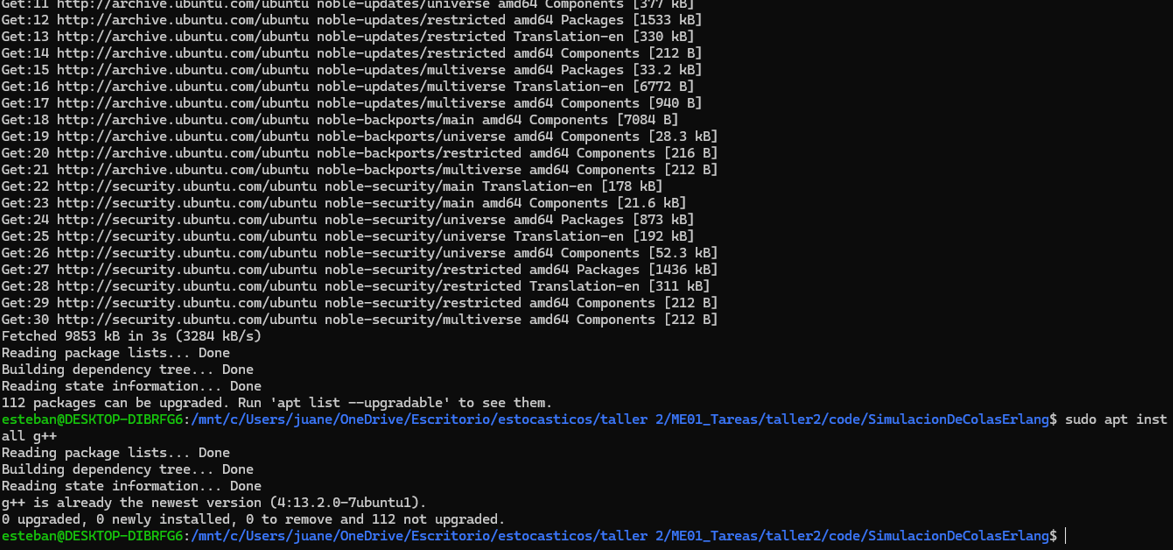
\includegraphics[width=0.8\textwidth]{images/manualUsuarioErlangBC_1.png}
    \caption{Proceso de instalación de g++}
    \label{fig:instalacion}
\end{figure}

Verificación de la instalación:
\begin{verbatim}
g++ --version
\end{verbatim}

\begin{figure}[H]
    \centering
    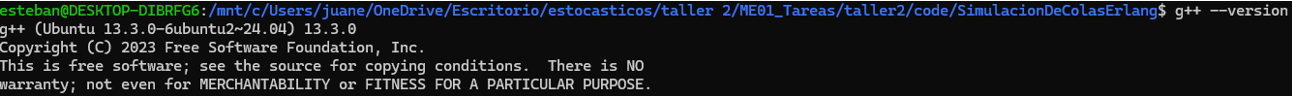
\includegraphics[width=0.8\textwidth]{images/manualUsuarioErlangBC_2.png}
    \caption{Verificación de la versión de g++}
    \label{fig:version}
\end{figure}

\subsubsection{Instalación de Ubuntu en WSL (Opcional)}
En caso de que se esté trabajando en windows hay varias alternativas para compilar y ejecutar el codigo c++. Acá presentamos una por medio de Ubuntu en WSL. Para instalarlo siga los siguientes pasos:

\begin{enumerate}
    \item Verificar/Activar característica WSL
    
    Ir al panel de control y seleccionar ``desistalar un programa`` en la sección de programas

    \begin{figure}[H]
    \centering
    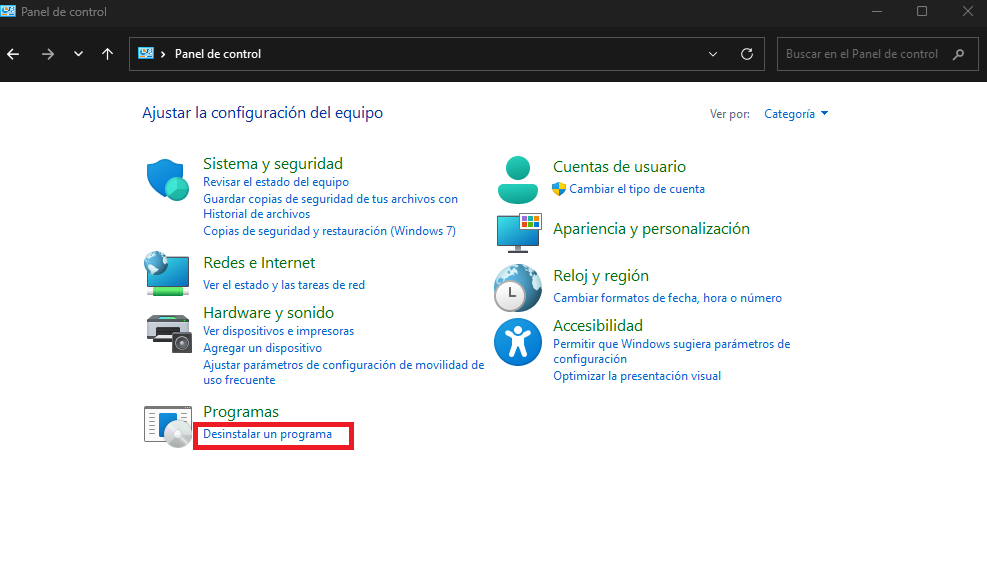
\includegraphics[width=0.8\textwidth]{images/manualUsuarioErlangBC_6.png}
    \caption{Panel de Control}
    \label{fig:version}
\end{figure}

A continuación a la izquierda encontrará ``Activar o desactivar las características de Windows`` al oprimirlo le abrirá una ventana donde debe verificar que la casilla ``Subsistema de Windows para Linux`` este seleccionada, en caso de no estarlo seleccionela

\begin{figure}[H]
    \centering
    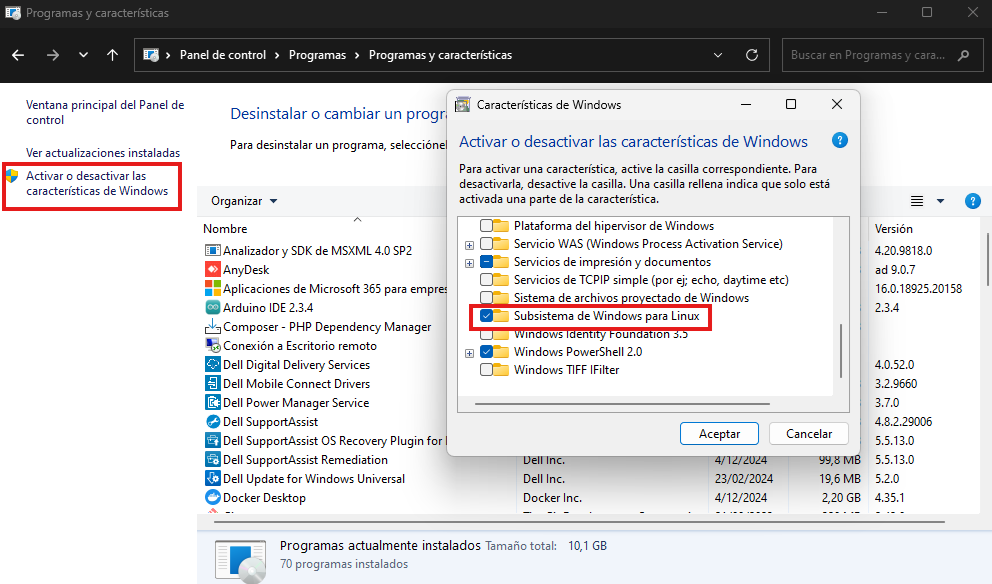
\includegraphics[width=0.8\textwidth]{images/manualUsuarioErlangBC_7.png}
    \caption{Características de Windows}
    \label{fig:version}
\end{figure}

    \item Instalación
    
    Vaya a Microsoft Store y busque Ubuntu, oprima la primera opción y despues ``Obtener``, acá se instalará. Pueden salir cuadros de dialogo para pedir permisos, oprima aceptar. Una vez finalizada la descarga abra el programa.

    \begin{figure}[H]
    \centering
    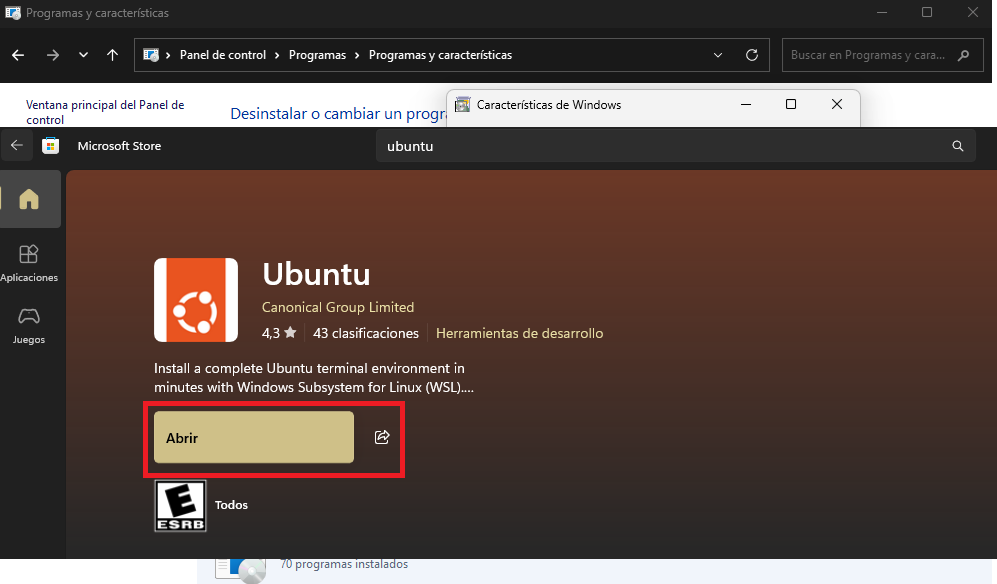
\includegraphics[width=0.8\textwidth]{images/manualUsuarioErlangBC_8.png}
    \caption{Microsoft Store}
    \label{fig:version}
\end{figure}

Finalmente siga los pasos para configurar el usuario y ejecute cualquier comando para verificar su correcto funcionamiento (Puede ussar el comando ls).

\begin{figure}[H]
    \centering
    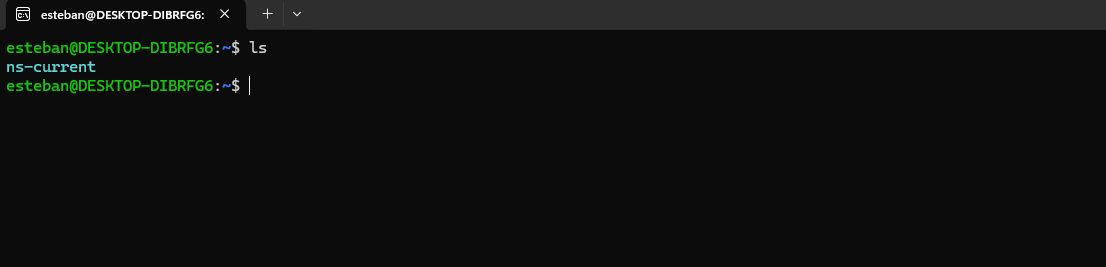
\includegraphics[width=0.8\textwidth]{images/manualUsuarioErlangBC_9.png}
    \caption{Instalación exitosa de Ubuntu en WSL}
    \label{fig:version}
\end{figure}

\end{enumerate}

\subsubsection{Configuración de parámetros}
Los parámetros de simulación se configuran en el archivo \texttt{param.txt} ubicado en \texttt{taller2/code/SimulacionDeColasErlang}. Los parámetros son:

\begin{itemize}
    \item \texttt{media\_entre\_llegadas}: Tiempo medio entre llegadas (float)
    \item \texttt{media\_atencion}: Tiempo medio de atención (float)
    \item \texttt{num\_esperas\_requerido}: Número de esperas a simular (integer)
    \item \texttt{modo}: Tipo de modelo Erlang (0 para B, 1 para C)
    \item \texttt{num\_servidores}: Cantidad de servidores (integer)
\end{itemize}

\begin{figure}[H]
    \centering
    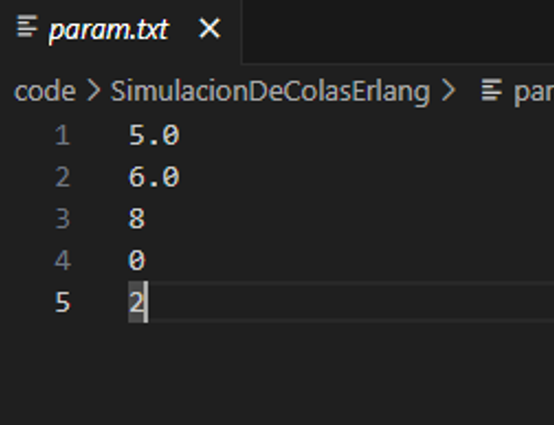
\includegraphics[width=0.8\textwidth]{images/manualUsuarioErlangBC_3.png}
    \caption{Ejemplo de archivo de parámetros}
    \label{fig:parametros}
\end{figure}

\subsubsection{Compilación y ejecución}
Proceso para compilar y ejecutar:

1. Compilación del programa:
\begin{verbatim}
g++ Sistema\ de\ Colas.cpp -o SistemaDeColas
\end{verbatim}

2. Ejecución del simulador:
\begin{verbatim}
./SistemaDeColas
\end{verbatim}

\begin{figure}[H]
    \centering
    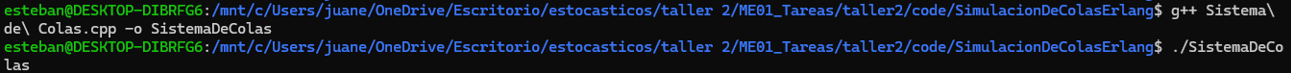
\includegraphics[width=0.8\textwidth]{images/manualUsuarioErlangBC_4.png}
    \caption{Proceso de compilación y ejecución}
    \label{fig:compilacion}
\end{figure}

\subsubsection{Resultados}
El programa genera un archivo \texttt{result.txt} con:

\begin{figure}[H]
    \centering
    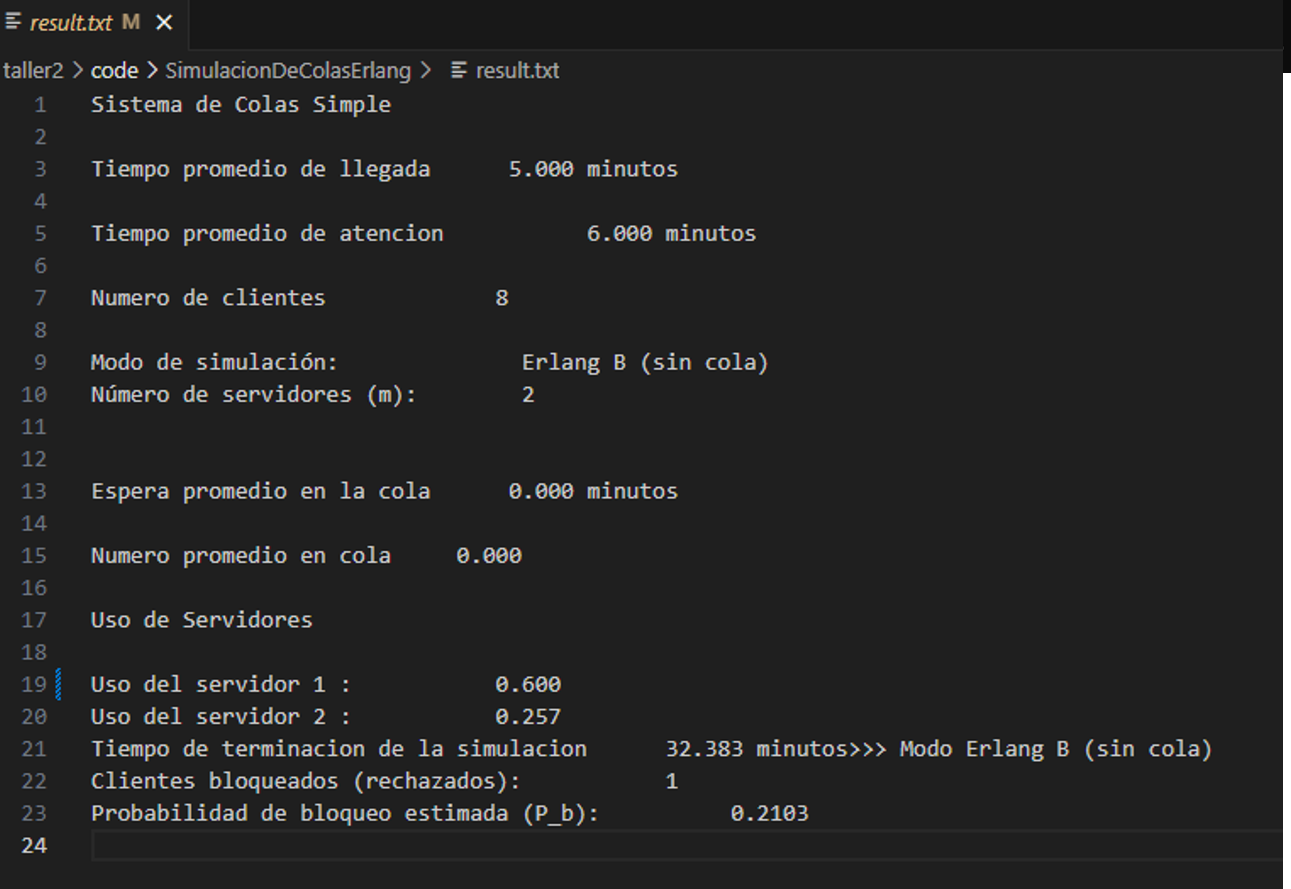
\includegraphics[width=0.8\textwidth]{images/manualUsuarioErlangBC_5.png}
    \caption{Ejemplo de archivo de resultados}
    \label{fig:resultados}
\end{figure}

La estructura del archivo incluye primero los parámetros de entrada, como los tiempos promedio de llegada y atención, el número de clientes simulados y la configuración de servidores. Luego, muestra los resultados principales, como la probabilidad de bloqueo, el uso de cada servidor y métricas de desempeño (tiempos de espera y ocupación). Finalmente, indica el tiempo total de simulación y el número de clientes rechazados. Este formato permite analizar rápidamente el comportamiento del sistema y la eficiencia de los recursos.

%---------------------------------------------------------------------------------
% Manual técnico ------------------------------------------------------------------
%---------------------------------------------------------------------------------

\section{Manual Técnico}

\subsection{Geo/Geo/m}\label{subsec:geogeo_m}

Simulador de un sistema de colas $(Geom/Geom/m):(FIFO/N/+ \infty)$ implementado en C++. El programa modela un sistema de colas con llegadas y servicios geométricos, múltiples servidores (m), capacidad finita (N) y disciplina FIFO.

\subsubsection{Prerequisitos}

\begin{itemize}
    \item Compilador C++ compatible con C++11 o superior
    \item Bibliotecas estándar: \texttt{stdio.h}, \texttt{stdlib.h}, \texttt{math.h}, \texttt{time.h}, \texttt{vector}
    \item Generador de números aleatorios proporcionado en \texttt{lcgrand.cpp}
    \item Sistema operativo: Windows/Linux/macOS
\end{itemize}

\subsubsection{Estructura del código}

El programa sigue una estructura modular con las siguientes componentes principales:

\begin{itemize}
    \item \textbf{Variables globales}:
    \begin{itemize}
        \item Parámetros del sistema (N, m, p, s, num\_slots)
        \item Estado del sistema (estado\_actual, servidores\_ocupados, cola\_length)
        \item Estadísticas (tiempo\_en\_estado[], clientes\_perdidos, clientes\_llegados)
    \end{itemize}
    
    \item \textbf{Funciones principales}:
    \begin{itemize}
        \item \texttt{main()}: Coordina el flujo del programa
        \item \texttt{inicializar()}: Prepara el sistema para la simulación
        \item \texttt{simular\_slot()}: Avanza la simulación un paso de tiempo
        \item \texttt{calcular\_estadisticas()}: Calcula métricas de desempeño
    \end{itemize}
    
    \item \textbf{Funciones auxiliares}:
    \begin{itemize}
        \item Generación aleatoria: \texttt{generar\_bernoulli()}, \texttt{generar\_binomial()}
        \item Cálculos matemáticos: \texttt{factorial()}, \texttt{potencia()}, \texttt{comb()}
        \item Modelo teórico: \texttt{geom\_geom\_m\_N\_p\_calc()}, \texttt{a\_func()}
    \end{itemize}
\end{itemize}

\subsubsection{Parámetros de la simulación}

Los parámetros se leen del archivo \texttt{paramGeo.txt} con el formato:

\begin{verbatim}
N m p s num_slots
\end{verbatim}

Donde:
\begin{itemize}
    \item \textbf{N}: Capacidad máxima del sistema (clientes)
    \item \textbf{m}: Número de servidores
    \item \textbf{p}: Probabilidad de llegada en un slot
    \item \textbf{s}: Probabilidad de finalización de servicio en un slot
    \item \textbf{num\_slots}: Duración de la simulación (slots)
\end{itemize}

\subsubsection{Salidas de la simulación}

El programa genera tres archivos de salida:

\begin{itemize}
    \item \texttt{estadisticas.txt}: Distribución de probabilidad del número de clientes en el sistema y probabilidad de bloqueo
    \item \texttt{comparacion\_teorica.txt}: Comparación entre resultados simulados y teóricos
    \item \texttt{resumen\_resultados.txt}: Métricas agregadas (utilización, promedio de clientes, throughput)
\end{itemize}

\subsubsection{Funciones principales}

\paragraph{\texttt{main()}}
\begin{itemize}
    \item Lee parámetros de \texttt{paramGeo.txt}
    \item Inicializa el sistema
    \item Ejecuta el bucle principal de simulación
    \item Coordina el cálculo y reporte de resultados
\end{itemize}

\paragraph{\texttt{simular\_slot()}}
\begin{itemize}
    \item Genera llegadas usando distribución Bernoulli(p)
    \item Genera salidas usando distribución Binomial(servidores\_ocupados, s)
    \item Actualiza el estado del sistema
    \item Registra estadísticas
\end{itemize}

\paragraph{\texttt{geom\_geom\_m\_N\_p\_calc()}}
Implementa el algoritmo para calcular las probabilidades de estado estacionario teóricas según el modelo Geom/Geom/m/N, basado en:
\begin{itemize}
    \item Thomas G. Robertazzi \textit{Computer Networks and Systems: Queueing Theory and Performance Evaluation Third Edition}
    \item 6.4 The Geom/Geom/m/N Queing system
\end{itemize}

\paragraph{\texttt{a\_func()}}
Función auxiliar que calcula $a_{i,j} \ 's$

\subsubsection{Compilación y ejecución}

Para compilar y ejecutar el simulador:

\begin{verbatim}
g++ sistemaGeoGeo.cpp -o sistemaGeoGeo 
./sistemaGeoGeo
\end{verbatim}

\subsubsection{Extensión del código}

Para modificar o extender el código:
\begin{itemize}
    \item Para cambiar el generador de números aleatorios, modificar \texttt{lcgrand.cpp}
    \item Para añadir nuevas métricas, extender \texttt{calcular\_estadisticas()}
    \item Para cambiar el modelo de llegadas/servicios, modificar \texttt{simular\_slot()}
\end{itemize}




%---------------------------------------------------------------------------------
% Exprimentación ------------------------------------------------------------------
%---------------------------------------------------------------------------------


\section{Experimentación}\label{sec:exp}



%---------------------------------------------------------------------------------
% Conclusiones ---------------------------------------------------------
%---------------------------------------------------------------------------------

\section{Conclusiones}\label{sec:concl}


%---------------------------------------------------------------------------------
% Recomendaciones ---------------------------------------------------------
%---------------------------------------------------------------------------------

\section{Recomendaciones}\label{secrecomen}





\section{Referencias}
\renewcommand{\refname}{}
\begin{thebibliography}{9}

\bibitem{ref} \label{ref:modSim} A. M. Law, *Simulation Modeling and Analysis*, 5th ed. 
New York, NY, USA: McGraw-Hill Education, Jan. 2014, ISBN 978-0-07-340132-4. 

\bibitem{ref} \label{ref:matSim} J. E. Ortiz T., “Modelos Matemáticos \& Simulación,”
 en *Apuntes de clase de la asignatura Modelos Estocásticos y Simulación en 
 Computación y Comunicaciones*, Departamento de Ingeniería de Sistemas e Industrial, 
 Universidad Nacional de Colombia, 2025. [En línea]. Disponible en: 
 \url{https://drive.google.com/file/d/1c886yU4SFk9A97DGWr8JHiF3nd2au1Ns/view?usp=sharing}

 \bibitem{ref} \label{ref:cimColas} J. E. UOrtiz, “Simulador del modelo de colas M/M/1,” 
 código fuente en C++ (archivo .rar), basado en la sección 
 1.4.4 de Averill M. Law, *Simulation Modeling and Analysis*, 
 th ed., McGraw-Hill, 2014. [En línea]. Disponible en: 
 \url{https://drive.google.com/file/d/1-Mo9hqPwOegwTpx0KP2tbD9sLTNSXefd/view?usp=sharing}



\end{thebibliography}

\end{document}